\chapter{MODELLO DIGITALE DEL TERRENO}
Prima di iniziare con la progettazione, bisogna creare un file DGN in cui il seed identifichi un foglio di lavoro 3D e dove il workflow utilizzato sia Openroads modeling. Dopo questa operazione è possibile creare un modello digitale del terreno, ovvero la ricostruzione di una parte di superficie terrestre a partire da un dato di origine.  Il modello digitale di terreno utilizzato è chiamato Digital Terrain Model (DTM) e comprende la superficie topografica (senza oggetti presenti sul terreno). Per inserire la cartografia come riferimento esterno bisogna inserire il comando Attach tools, e cliccando sulla vista fit view sarà possibile visualizzare il terreno nella sua completezza. Al fine di creare un DTM è necessario partire con la realizzazione di un filtro grafico, che è possibile creare nella sezione Terrain con il comando From Graphical Filter. Con lo stesso procedimento creiamo un filtro sia per le curve di livello che per i punti quotati. Successivamente bisogna creare un perimento (a) contenente i filtri creati e che permetta di attivare e visualizzare a video la vista triangolare del terreno (b) con il comando Max triangle lenght (all’aumentare dei triangoli aumenta la precisione). Grazie alla possibilità di ruotare il nostro DTM possiamo osservare il nostro modello 3D in varie angolazioni.

\begin{figure}[h]
  \begin{subfigure}{.5\textwidth}
  \centering
    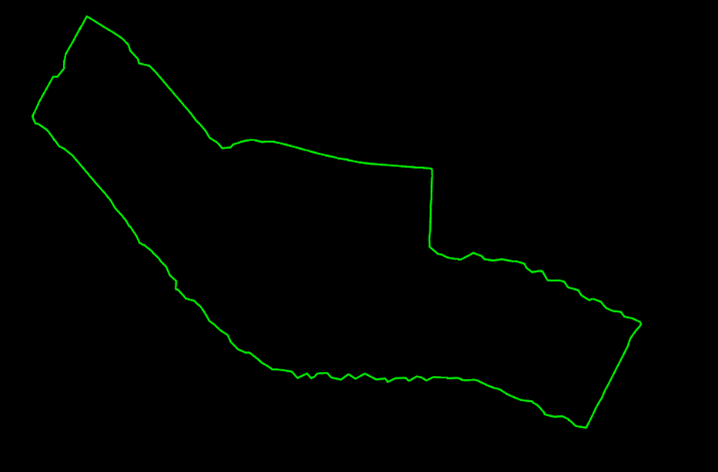
\includegraphics[width=0.8\linewidth]{Figures/perimetro}
    \caption{perimetro}
  \end{subfigure}%
  \begin{subfigure}{.5\textwidth}
  \centering
    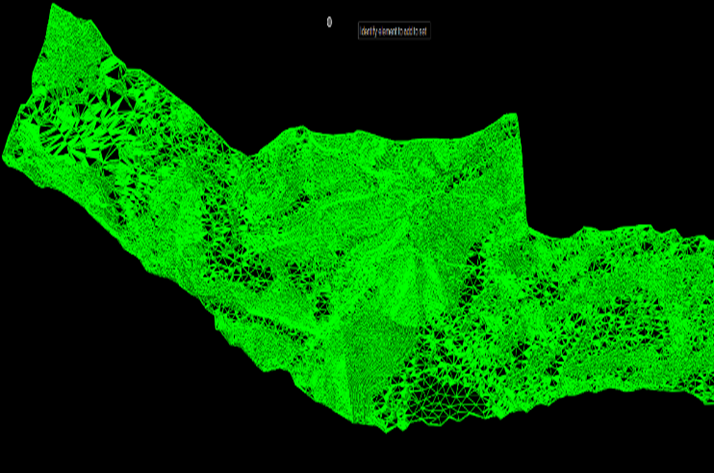
\includegraphics[width=0.8\linewidth]{Figures/vista triangolare}
    \caption{vista triangolare}
  \end{subfigure}
  \caption{}
\end{figure}